\section{Experiment Results \& Discussion}
\label{sec:experiments}

We first separated or data in train, validation and test datasets,
comprising of respectively 70\%, 20\% and 10\% of the total data.
We broke our data in the time axis, so the validation and test data are referents to the later days instead of different pages.
After we separated the dataset we end up with, 559 samples for the training set, 159 samples for the validation set and 79 samples for the test set.

The code of the experiments were written in python with the module for neural network keras using the tensorflow as back-end.
The models were ran in a intel core i7-6700k, with 16GB of memory and Geforce-980 Ti.

Due to memory constraints we decided to limit the number of pages on the test data, from 145063 to 50000.

\subsection{MLP}

The MLP model receives an input composed of an unique identifier of the wikipage accessed,
the number of days passed since the first measurement was collected,
and the number of visits from the last 7 days.

The MLP is built with one input layer of size 1024, two hidden layers of size 1024 and a output layer of size 1.
The optimizer chosen was Adam with learning rate of $10^{-7}$ during 20 epochs and using batch size of 1000.
The learning rate does not decrease over time. The loss graph can be seen on figure \ref{fig:model_1_loss}.

\begin{figure}
	\centering
	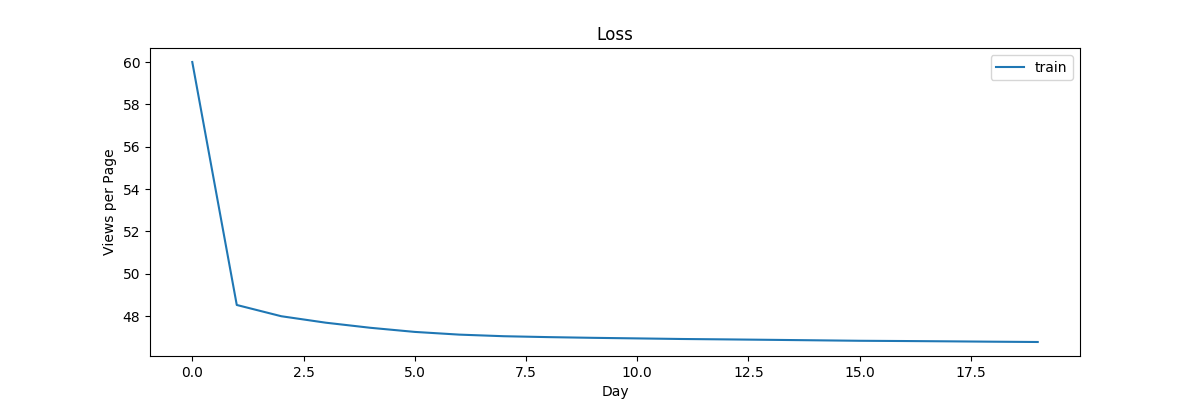
\includegraphics[width=\linewidth]{model_1_loss.png}
	\caption{Loss graph from model MLP\label{fig:model_1_loss}}
\end{figure}

\begin{figure}
	\centering
	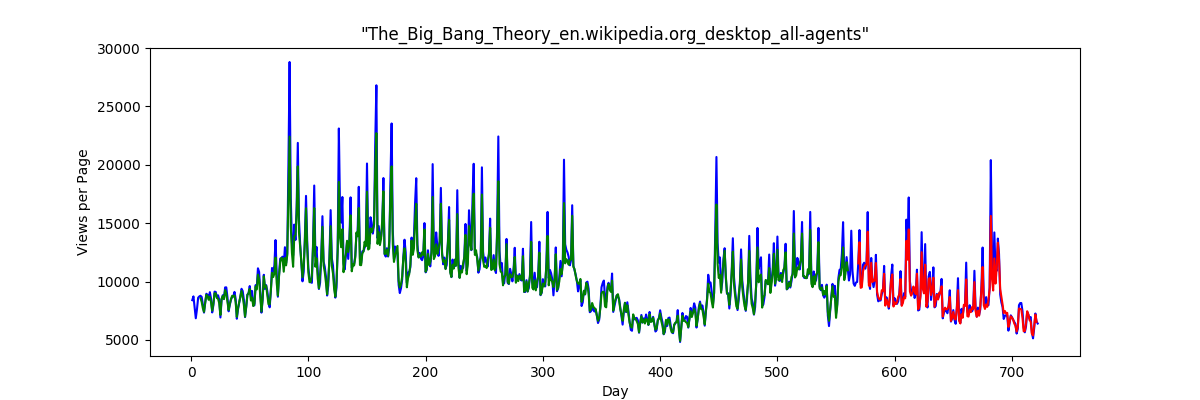
\includegraphics[width=\linewidth]{model_1_TBT.png}
	\caption{Plot of the values of visits per day compared to the prediction of MLP of the page The Big Bang Theory (en) of all desktops\label{fig:model_1_TBT}}
\end{figure}

\begin{figure}
	\centering
	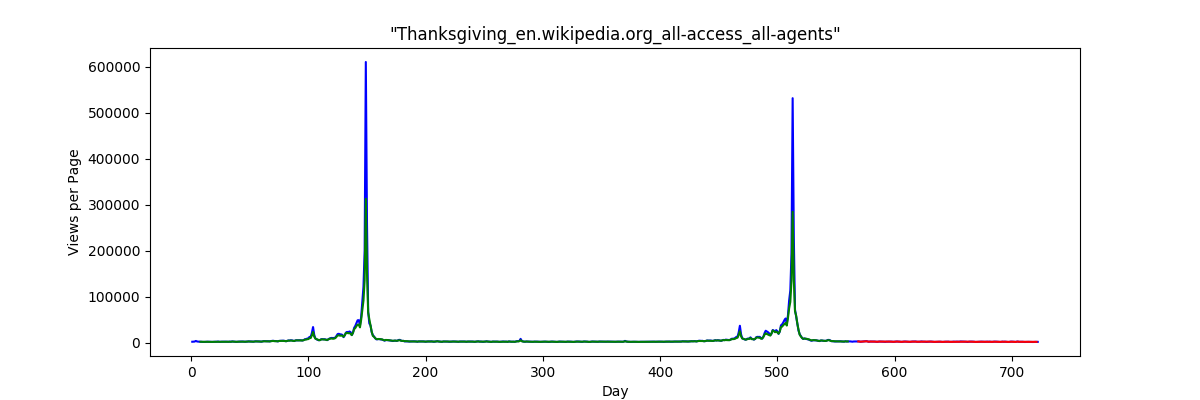
\includegraphics[width=\linewidth]{model_1_TG.png}
	\caption{Plot of the values of visits per day compared to the prediction of MLP of the page Thanksgiving (en) of all desktops\label{fig:model_1_TG}}
\end{figure}

It is easy to see on figure \ref{fig:model_1_TBT} that the model achieved a pretty good accuracy on the maintaining close to the behavior of the curve,
however the model undershoot the largest spikes, which probably leads to the biggest percentage of lost score.

The graph for thanksgiving is a very odd one, the only spikes happens on thanksgiving day,
which is once a year and does not occur neither on validation data or test data,
leaving the hardest prediction to appear only on training data.

\subsection{LSTM-stateless}

The LSTM model only uses as input, the page id,
the number of days pass the first measurement and the last count of visits of that page.

The LSTM model uses 4 layers of LSTM cells of size 256, a normalization batch,
two fully connected layers of size 1024 with ReLU as activation function and an output layer.
parallel to the LSTM layer there is a fully connected layer of size 1024 to try improving the use of recent data,
a batch normalization is also used after the fully connected layer too.

The batch normalization layers are used to contain the exploding gradients of deeper neural networks,
as well as the ReLU activation function. The Adam optimizer was chosen using learning rate of $10^-5$,
whiteout learning rate decay, the model was trained during 5 epochs with batch size of 1000.
The loss curve from the model training is displayed on figure \ref{fig:model_2_loss}.

\begin{figure}
	\centering
	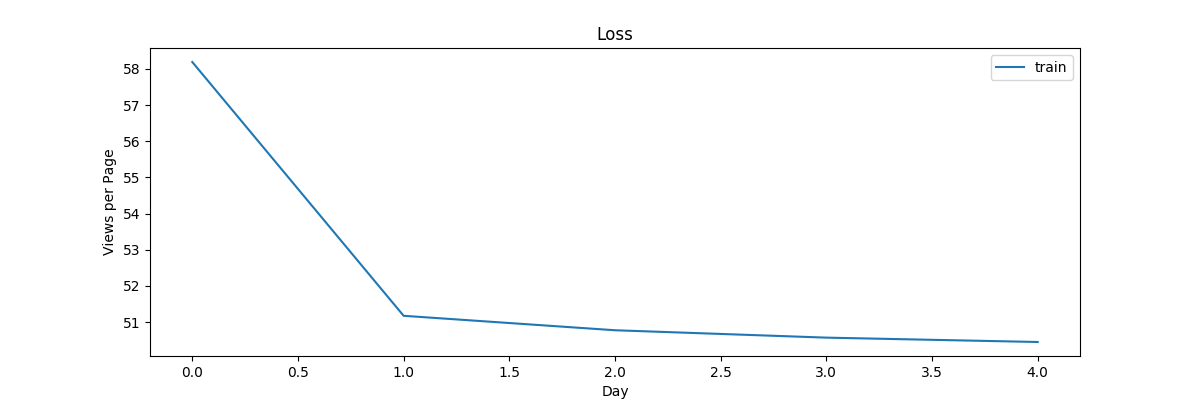
\includegraphics[width=\linewidth]{model_2_loss(stateless).png}
	\caption{Loss graph from model LSTM\label{fig:model_2_loss}}
\end{figure}

\begin{figure}
	\centering
	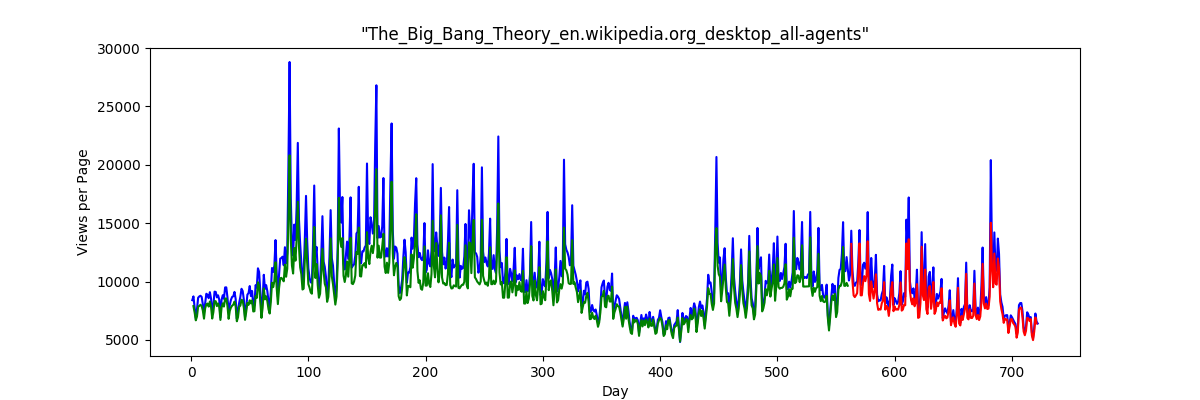
\includegraphics[width=\linewidth]{model_2_TBT(stateless).png}
	\caption{Plot of the values of visits per day, of the page The Big Bang Theory (en) of all desktops\label{fig:model_2_TBT}}
\end{figure}

\begin{figure}
	\centering
	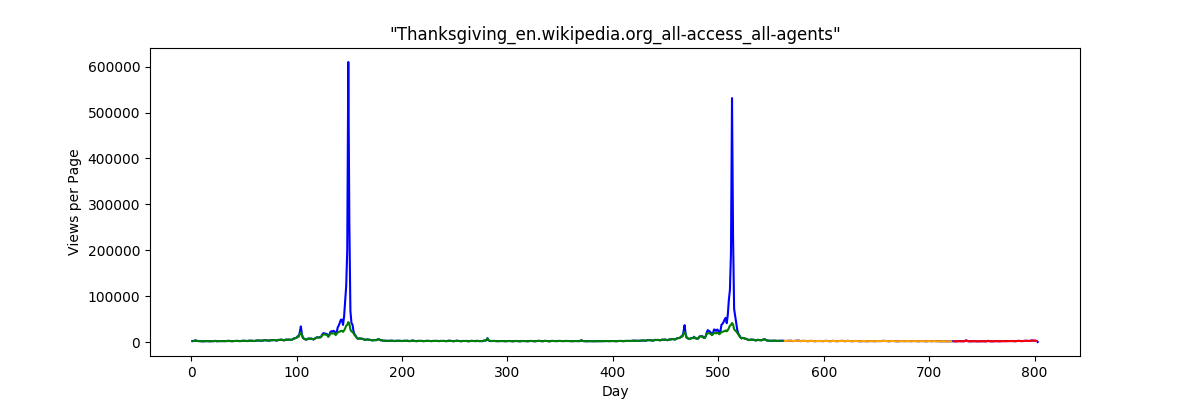
\includegraphics[width=\linewidth]{model_2_TG(stateless).png}
	\caption{Plot of the values of visits per day, of the page Thanksgiving (en) of all desktops\label{fig:model_2_TG}}
\end{figure}

the figure \ref{fig:model_2_TBT} shows that the LSTM model also follows the general format of the visit graph like the MLP model, however it undershoots not only the high spikes but, also some lower and more plateau segments.
which increases the loss value of the model.

On the figure \ref{fig:model_2_TG} it is possible to see that the LSTM model has a lot of difficult to follow the hight spikes from some pages.

\subsection{LSTM-stateful}